% ******************************************************************************
\section{Adding images}
% ******************************************************************************

% new slide
\begin{frame}[fragile]\small
  \frametitle{How to produce a slide with \textbf{itemize} environment}
    \begin{verbatim}
% new slide
\frame{
 \frametitle{Introduction}
   \begin{itemize}
     \item <1-> I hope you (as I do) find \LaTeX{} as a cool 
                and very useful tool
     \item <2-> For more information, do not forget to take a 
                look at \url{http://www.latex-project.org/}
     \item <3-> And at this place 
                \url{http://latex.simon04.net/} 
                you will find some themes for \textb{Beamer}
     \end{itemize}
}  
\end{verbatim}
\end{frame}

% new slide
\frame{
  \frametitle{Output of the previous slide}
       \begin{itemize}
            \item <1-> I hope you (as I do) find \LaTeX{} as a cool and very useful tool
            \item <2-> For more information, do not forget to take a look at \url{http://www.latex-project.org/}
            \item <3-> And at this place \url{http://latex.simon04.net/} you will find some themes for \textbf{Beamer}
        \end{itemize}
}

% new slide
\begin{frame}[fragile]\tiny
  \frametitle{How to produce a slide with an image}
    \begin{verbatim}
% new slide
\frame{
 \frametitle{Introduction}
    % add images to the slide
    % the image is titled "barplotNumberBinsPerHeuristic.pdf"
    % note that the ".pdf"is not required 
    % (unless there exist another image with the same name but 
    % with different format, such ".png" for example)
    % Do not forget to add the full path of the image
    \begin{center} 
      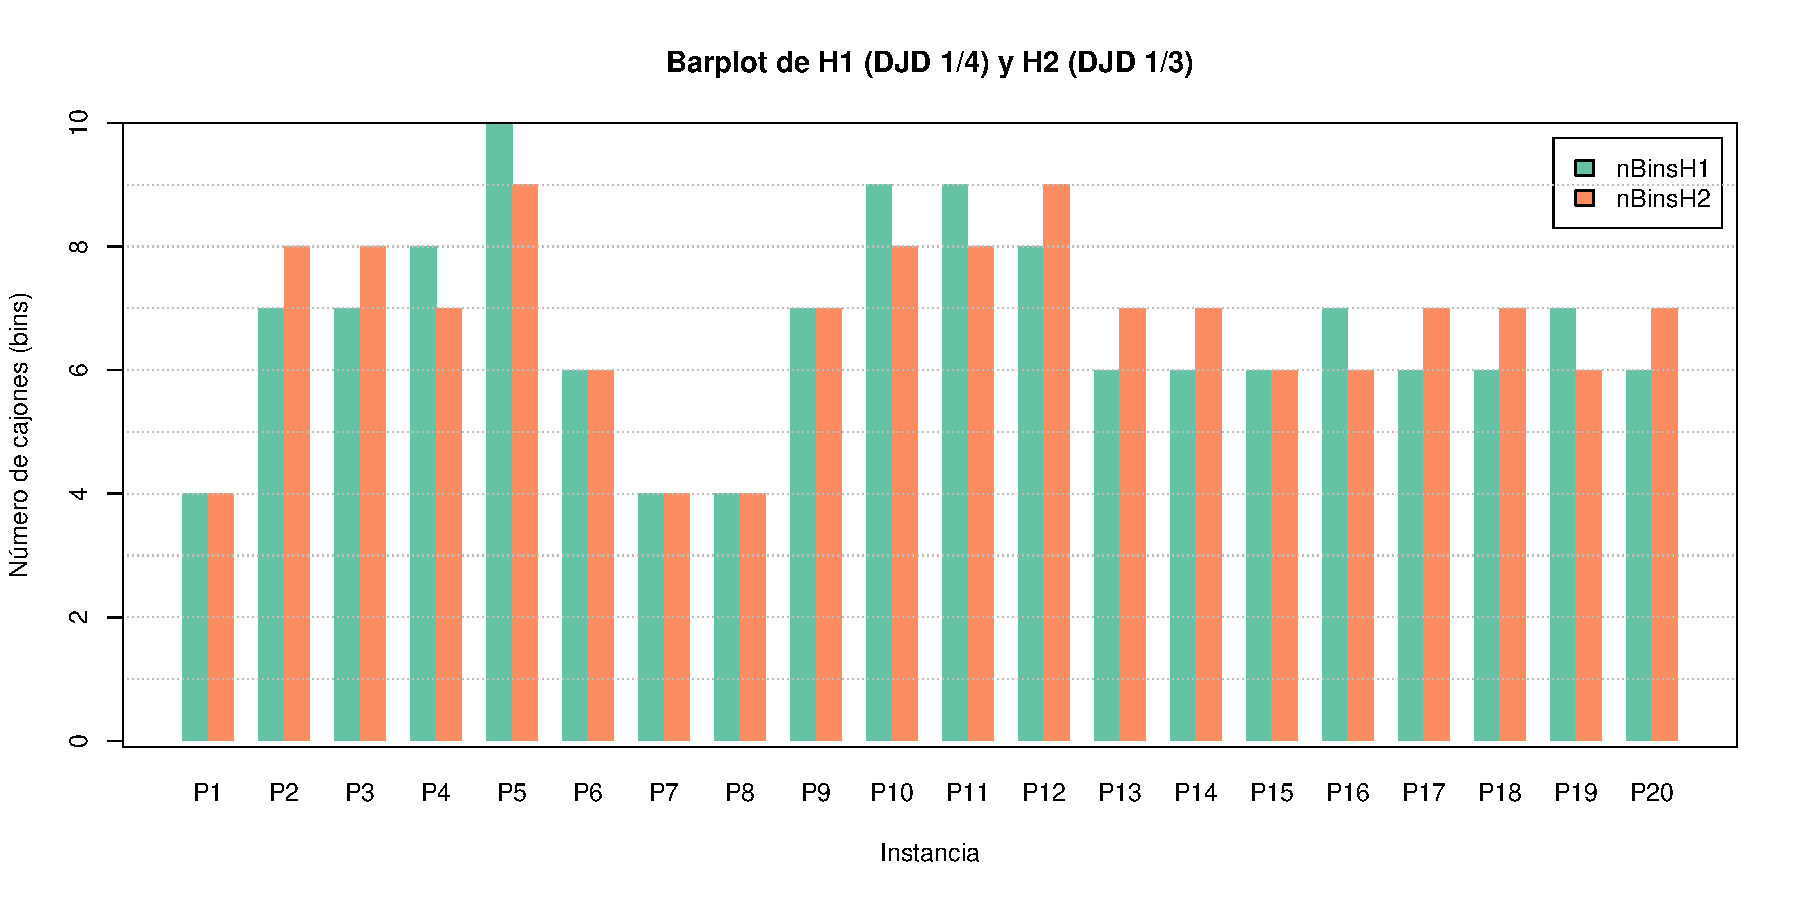
\includegraphics[width=0.8\textwidth]{images/introduction/barplotNumberBinsPerHeuristic}    
    \end{center}  
}
\end{verbatim}
\end{frame}


% new slide
\frame{
  \frametitle{Figure 1 (Output of the previous slide)}
    % add images to the slide
    \begin{center} 
        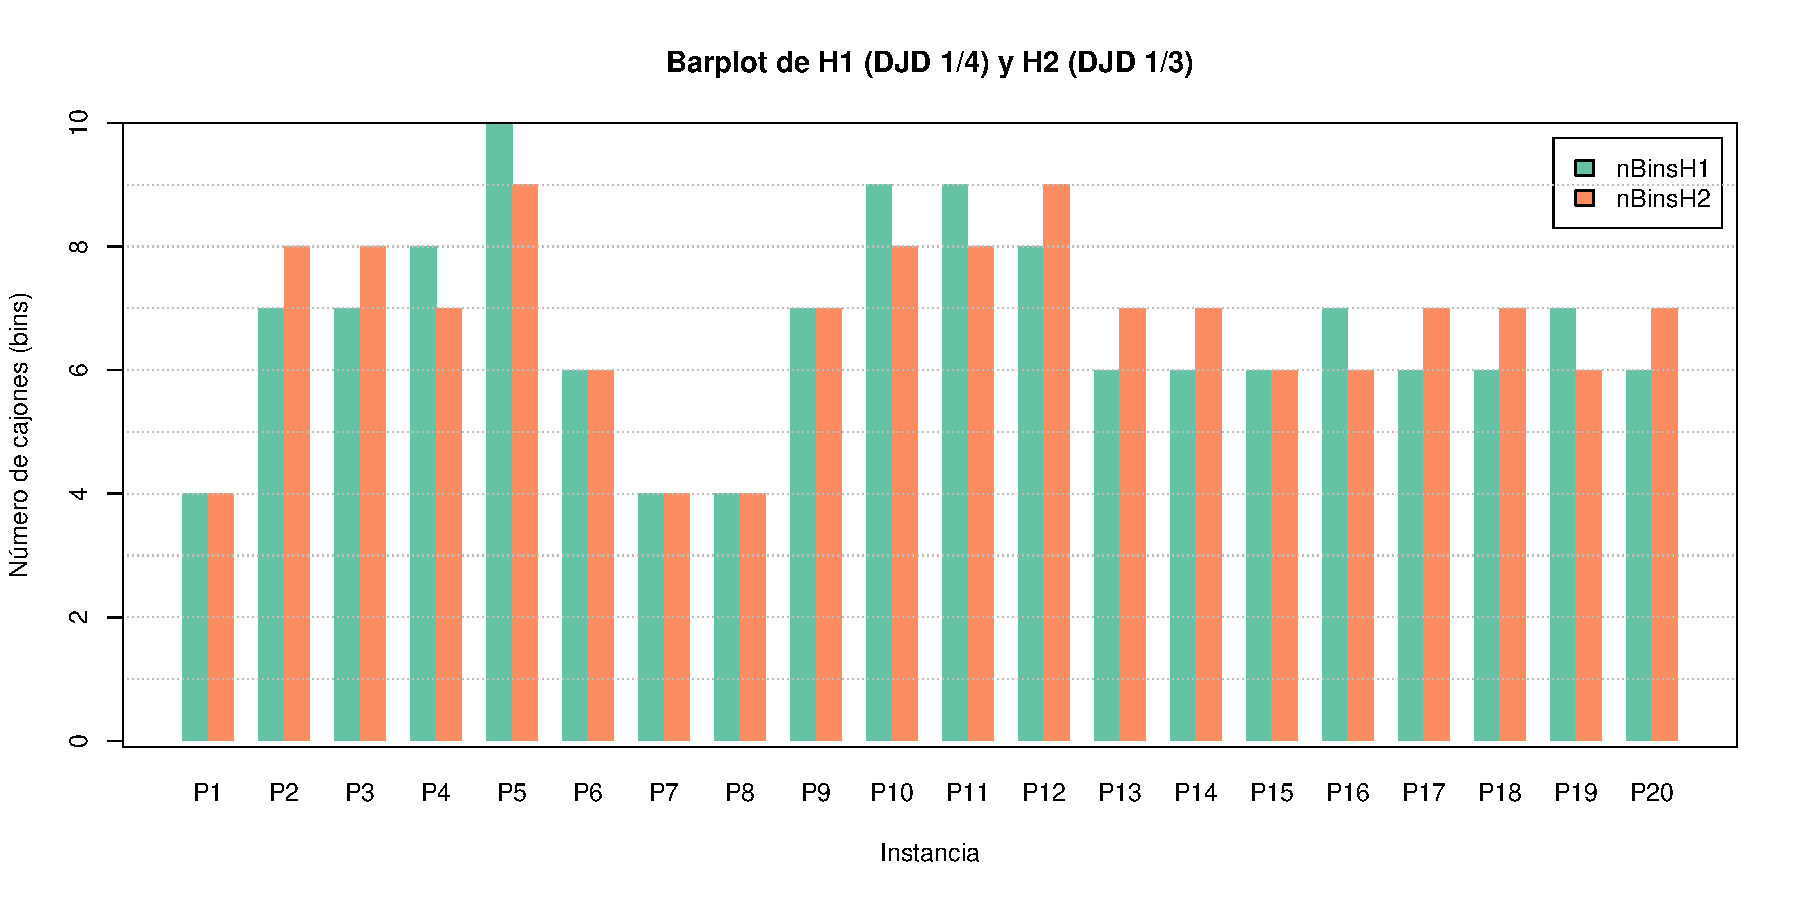
\includegraphics[width=0.99\textwidth]{images/introduction/barplotNumberBinsPerHeuristic}    
    \end{center}  
}

% new slide
\frame{
  \frametitle{Figure 2}
    % add images to the slide
    \begin{center} 
        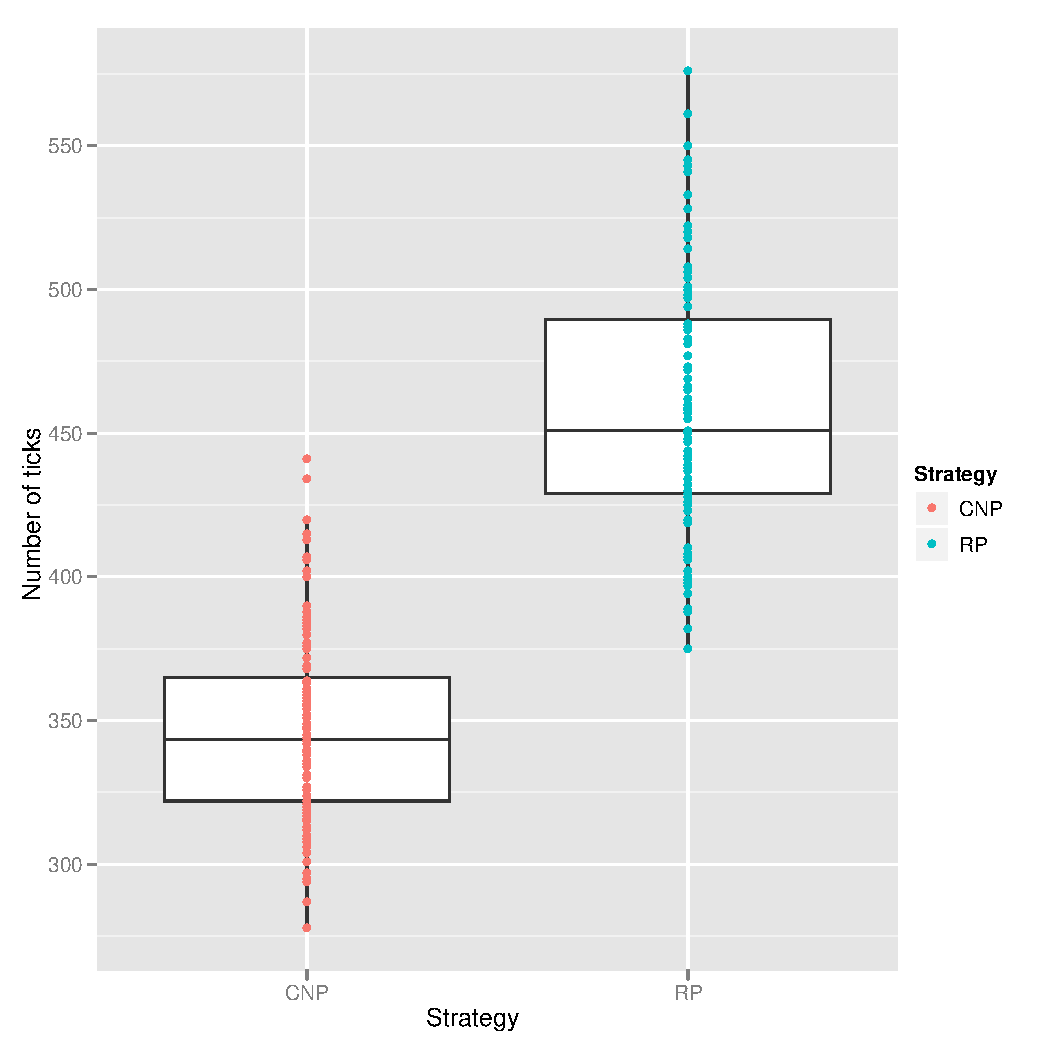
\includegraphics[width=0.6\textwidth]{images/introduction/boxplotTicks}    
    \end{center}  
}

% new slide
\frame{
  \frametitle{Additional notes 1}
       \begin{itemize}
            \item <1-> Please do not forget to take a look at the source code in order to learn how it works
            \item <2-> I've commented the most and critical parts of \textbf{beamerExample.tex} to help in the interpretation of the code
        \end{itemize}
}

% new slide
\frame{
  \frametitle{Additional notes 2}
       \begin{itemize}
            \item <1-> Each .tex file is just to show that you can \textit{split} your presentation into \textbf{sections}
            \item <2-> I prefer to work this way because I find it more organized and with less clutter it boost my understanding of the final PDF file without having to compile a lot of intermediary PDF files
            \item <3-> Always comment your code for further references and I suggest to keep managing your \textbf{sections} as individual .tex files
        \end{itemize}
}

% new slide
\frame{
  \frametitle{More examples | Figure 1}
    % add images to the slide
    \begin{center} 
        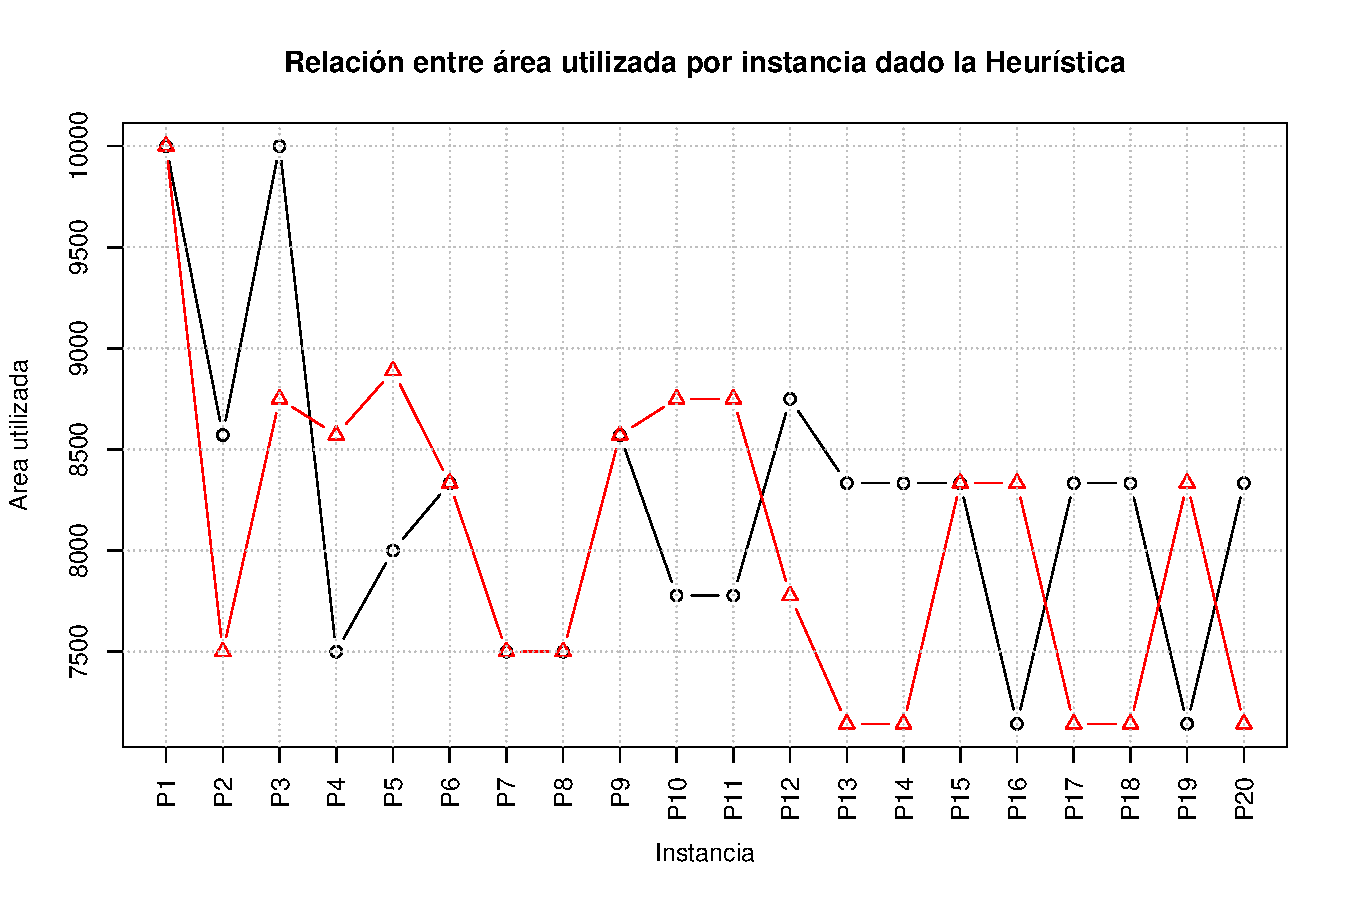
\includegraphics[width=0.9\textwidth]{images/addingImages/matplotAreaUsed}    
    \end{center}  
}

% new slide
\frame{
  \frametitle{More examples | Figure 2}
    % add images to the slide
    \begin{center} 
        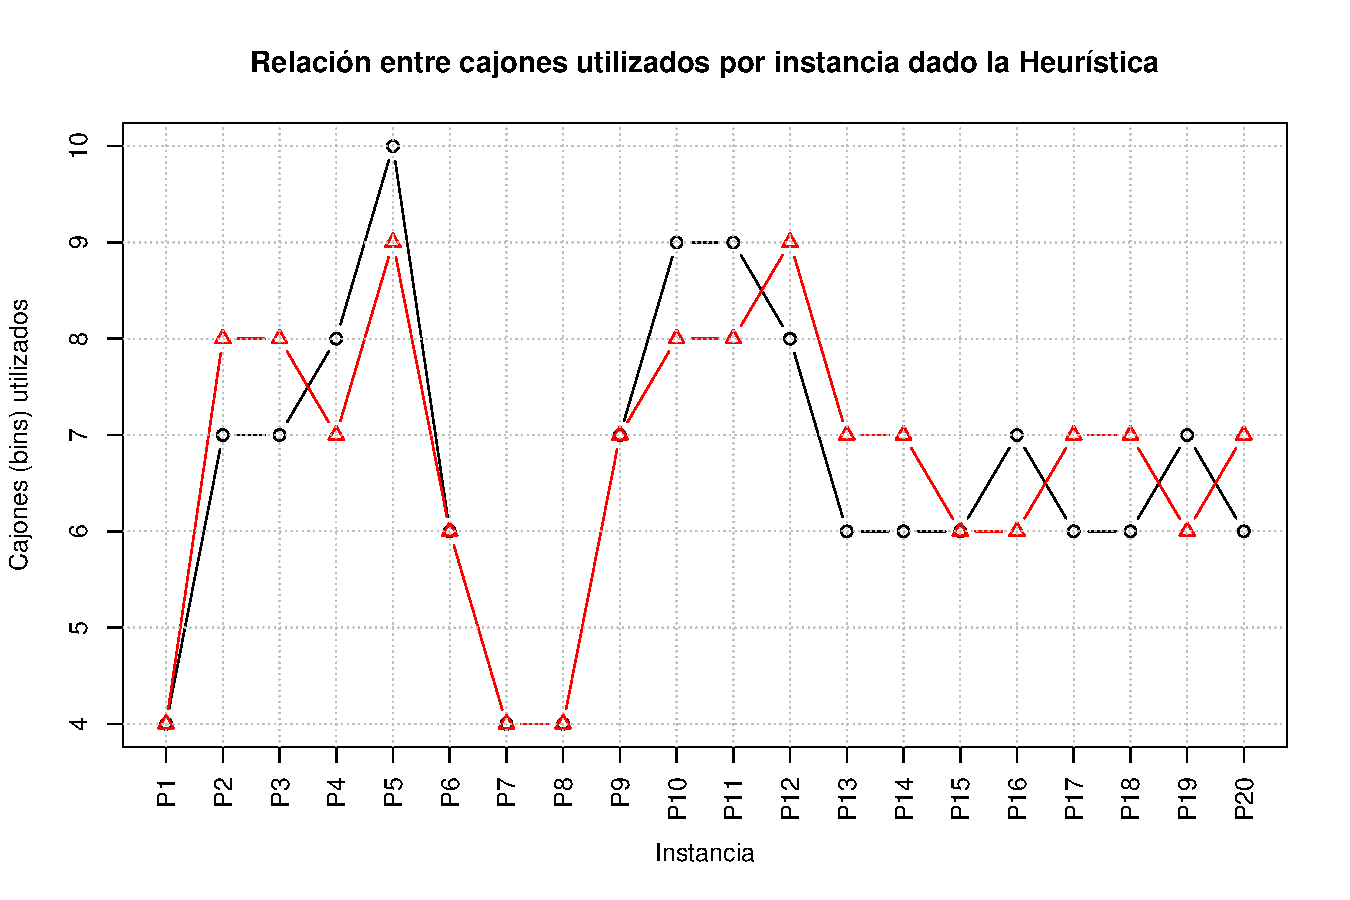
\includegraphics[width=0.9\textwidth]{images/addingImages/matplotNumberOfBins}    
    \end{center}  
}

% new slide
% Comparison of matplotAreaUsed and matplotNumberOfBins
\begin{frame}
    \frametitle{More examples | showing two images in the same slide}
	\begin{columns}[c]
	% FIRST IMAGE
	\column{2.15in}
		\framebox{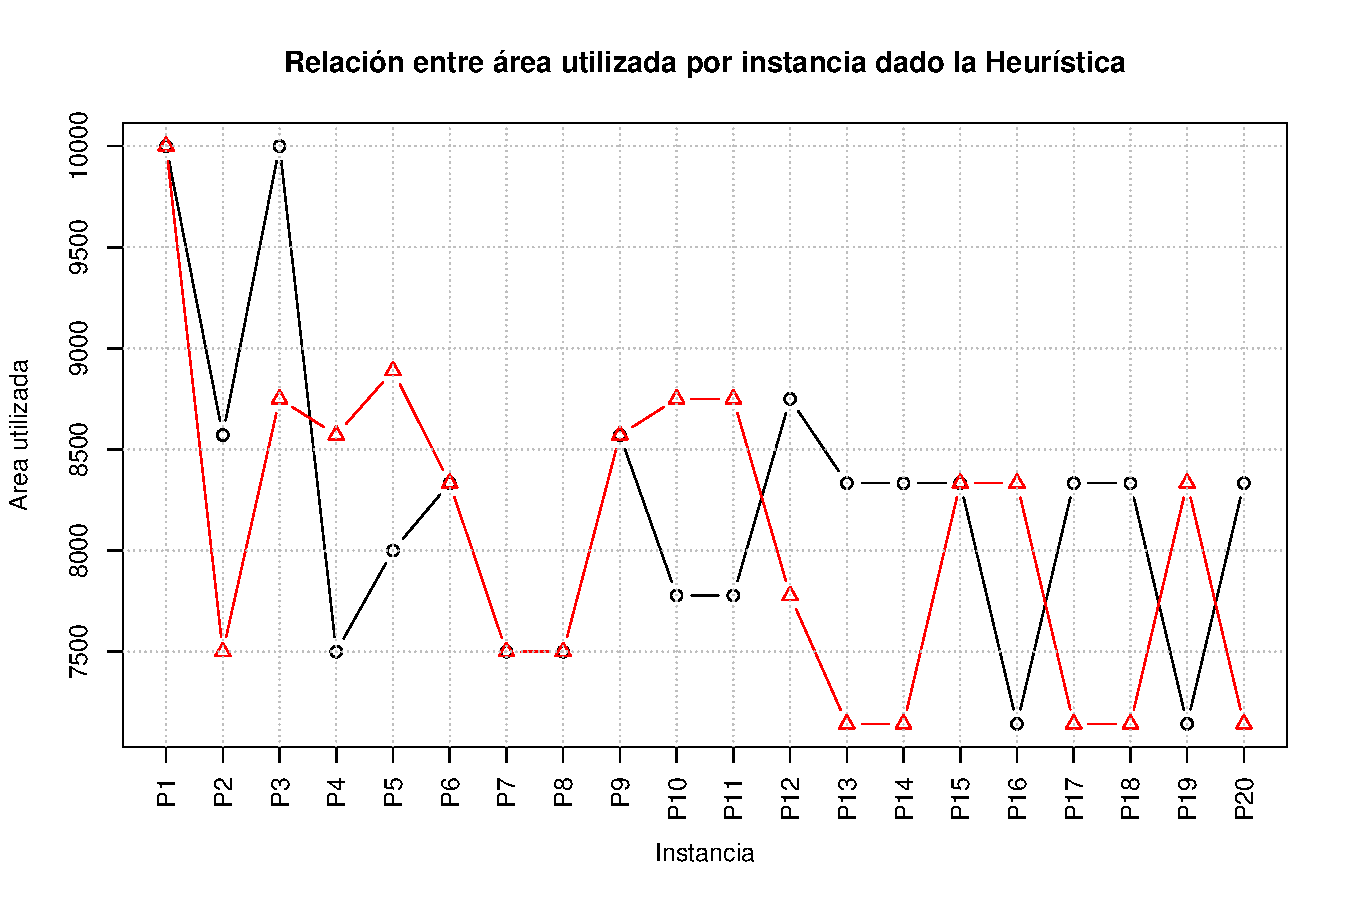
\includegraphics[width=2.2in]{images/addingImages/matplotAreaUsed}}
	% SECOND IMAGE 
	\column{2.4in}
		\framebox{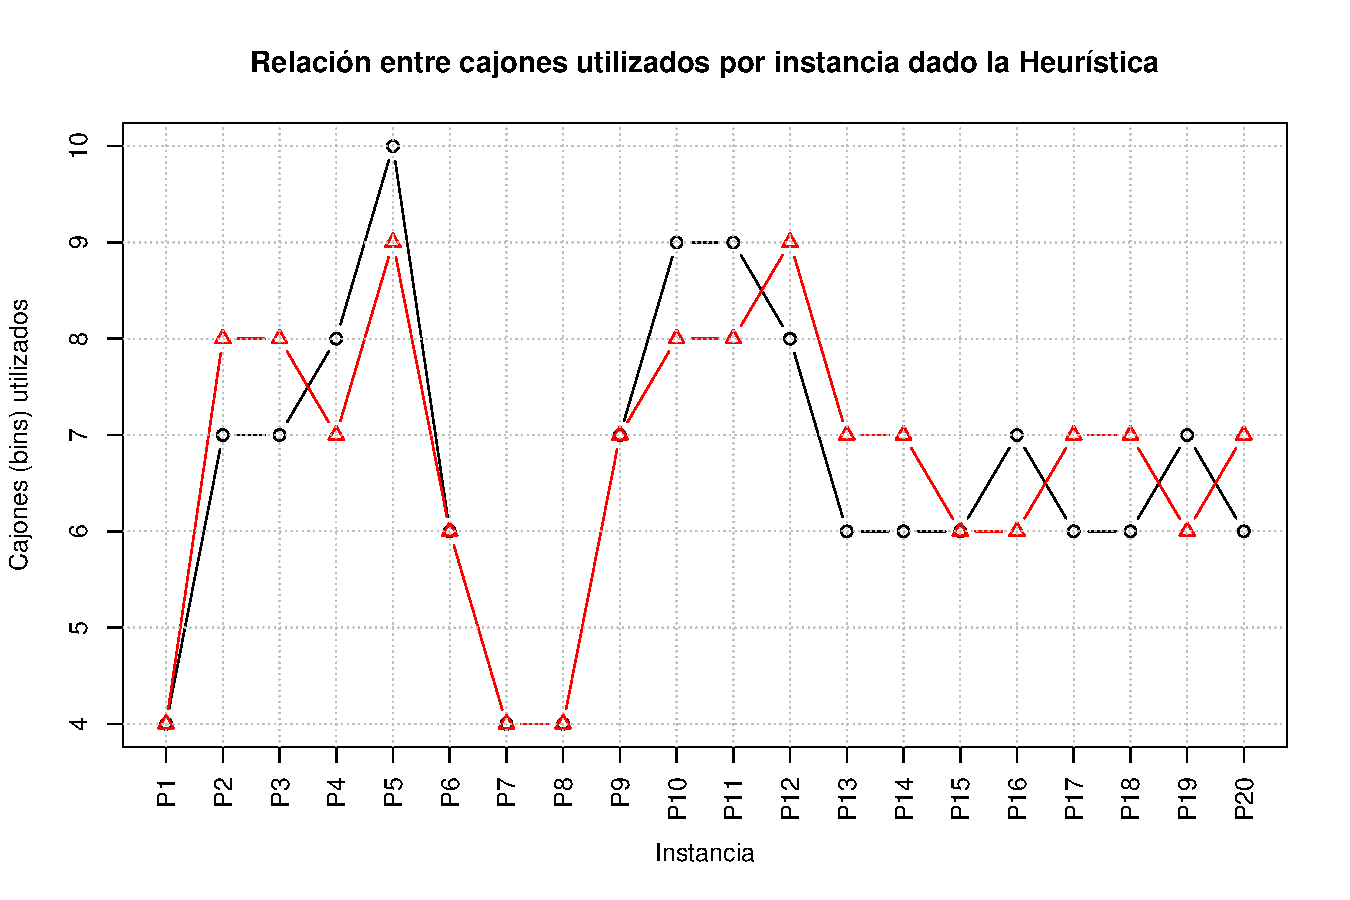
\includegraphics[width=2.2in]{images/addingImages/matplotNumberOfBins}}
	\end{columns}
\end{frame}


